% Gemini theme
% https://github.com/anishathalye/gemini
%
% We try to keep this Overleaf template in sync with the canonical source on
% GitHub, but it's recommended that you obtain the template directly from
% GitHub to ensure that you are using the latest version.

\documentclass[final]{beamer}

% ====================
% Packages
% ====================

\usepackage[T1]{fontenc}
\usepackage{lmodern}
% \usepackage[size=custom,width=70,height=122,scale=1]{beamerposter}
\usepackage[orientation=portrait, size=a0,scale=1.2]{beamerposter}
\usetheme{gemini}
\usecolortheme{gemini}
\usepackage{graphicx}
\usepackage{booktabs}
% \usepackage{multicol}
\usepackage{tikz}
\usepackage{pgfplots}
\pgfplotsset{compat=1.14}

\usepackage{tabularx}
\usepackage{booktabs, multirow}
\usepackage{subcaption}
\usepackage{diagbox}
\usepackage{caption}
\usepackage{multicol}
% \usepackage[table]{xcolor}
\usepackage{xcolor,colortbl}
\usepackage{adjustbox}

\usepackage{soul}
\usepackage[normalem]{ulem}
% ====================
% Lengths
% ====================

% If you have N columns, choose \sepwidth and \colwidth such that
% (N+1)*\sepwidth + N*\colwidth = \paperwidth
\newlength{\sepwidth}
\newlength{\colwidth}
\setlength{\sepwidth}{0.025\paperwidth}
\setlength{\colwidth}{0.3\paperwidth}

\newcommand{\separatorcolumn}{\begin{column}{\sepwidth}\end{column}}

% ====================
% Title
% ====================

\title{Modeling Syntactic-Semantic Dependency Correlations in Semantic Role Labeling Using Mixture Models}

\author{Junjie Chen \inst{1} \and Xiangheng He \inst{2} \and Yusuke Miyao \inst{1}}

\institute[shortinst]{\inst{1} The University of Tokyo \samelineand \inst{2} Imperial College London}

% ====================
% Footer (optional)
% ====================

% \footercontent{
%   \href{https://www.example.com}{https://www.example.com} \hfill
%   ABC Conference 2025, New York --- XYZ-1234 \hfill
%   \href{mailto:alyssa.p.hacker@example.com}{alyssa.p.hacker@example.com}}
% (can be left out to remove footer)

% ====================
% Logo (optional)
% ====================

% use this to include logos on the left and/or right side of the header:
\logoleft{
\includegraphics[height=7cm]{images/utokyo logo.jpg}}
\logoright{
\includegraphics[height=7cm]{images/IC logo.png}}

% ====================
% Body
% ====================

\begin{document}

\begin{frame}[t]
\vspace{-.5\baselineskip}
\begin{columns}[t]
\separatorcolumn

\begin{column}{\colwidth}
    \begin{block}{Introduction}
We study the syntactic-semantic dependency correlation through the mutual information gain of SSDP hop patterns.
% \setlist{nolistsep}
\begin{itemize}
    % \item Syntactic dependencies: Head$\rightarrow$Dependent relations.
    % \item Semantic dependencies: Predicate$\rightarrow$Argument relations. We denote the relation type as semantic labels.
    \vspace{-0.8cm}
    \item Semantic label: relation type (e.g., A0) of semantic dependencies
    \item SSDP: Shortest Syntactic Dependency Path connecting predicate-argument pairs
    \item Hop pattern: the transition pattern of SSDP
\end{itemize}
\begin{figure}
    \centering
    \captionsetup{justification=centering}
    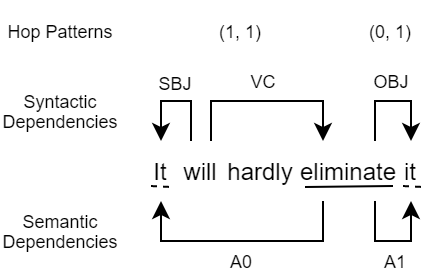
\includegraphics[width=0.7\textwidth]{images/syn-sem-dep-example.png}
    \caption{Example semantic dependencies, SSDP of the semantic dependencies, and hop patterns. Solid lines underline predicates and dash lines underline arguments.}
    \label{fig:syn-sem example}
\end{figure}
% Hop patterns distinguish the two semantic dependencies with the same predicate-argument pair.\\
% \vspace{0.5cm}
% \textbf{Hypothesis: Different hop patterns have unique distributions of semantic labels.}
Intuitions:
\begin{itemize}
\vspace{-1cm}
    \item Semantic dependencies are modeled as a distribution of the predicate and the argument \cite{dozat-manning-2018-simpler, strubell-etal-2018-linguistically, he-etal-2018-syntax}
    \item Semantic parsers are vulnerable to semantic dependencies (Figure \ref{fig:syn-sem example}) that have different semantic labels but share the same predicate and argument
    \item Hop patterns can distinguish between the two semantic dependencies
\end{itemize}

\textbf{Hypothesis: Different hop patterns have unique distributions of semantic labels}


\end{block}
    % \begin{block}{Contributions}
% \textbf{Backgrounds}
% \begin{itemize}
%     \item Semantic dependencies $(p, a, r)$ as a conditional distribution $P(r|p, a)$ of semantic labels $r$ for all predicates $p$ and arguments $a$ \cite{dozat-manning-2018-simpler}. 
%     \begin{itemize}
%         \item Cannot utilize the syntactic-semantic dependency correlation.
%     \end{itemize}
%     \item The dependency correlation as a co-occurrence bias between syntactic and semantic dependencies \cite{he-etal-2018-syntax}.
%     \begin{itemize}
%         \item The co-occurrence bias is hardcoded into heuristics, making the heuristics language-dependent.
%     \end{itemize}

% \textbf{Intuitition}

% Contributions:
\begin{itemize}
\vspace{-0.5cm}
    \item Interpreting the dependency correlation using the information gain of hop patterns.
    \item Proposing a mixture model based method learning the dependency correlation.
\end{itemize}
\end{block}
    \begin{exampleblock}{Proposal Overview}
We propose a mixture model-based semantic parser (MM) that
\begin{itemize}
    \vspace{-0.5cm}
    \item Clusters hop patterns with similar semantic label distributions using mixture weights
    \item Decouples semantic label distributions for different hop patterns using component distributions
\end{itemize}
% \textbf{} and \textbf{}

\begin{figure}
    \centering
    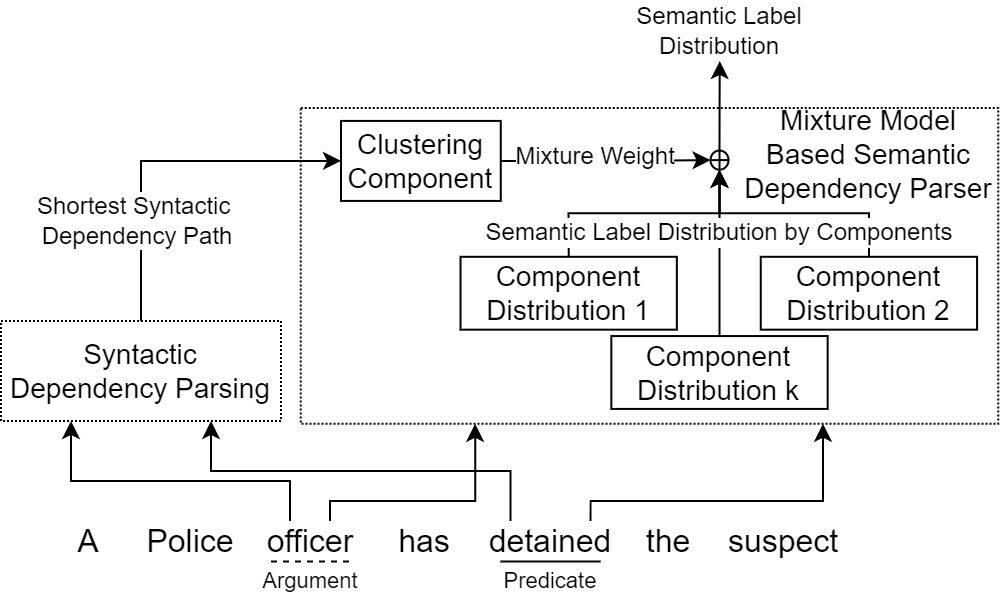
\includegraphics[width=0.95\textwidth]{images/mm-illustra.drawio.png}
    \caption{Illustration of the proposed model.}
    % \label{fig:my_label}
\end{figure}



\end{exampleblock}
      \begin{block}{References}

    % \nocite{*}
    \footnotesize{\bibliographystyle{plain}\bibliography{anthology}}

  \end{block}
\end{column}

\separatorcolumn

\begin{column}{2\colwidth}
    \begin{block}{Correlation: Semantic label distributions differ by hop patterns}
% \vspace{-.2\baselineskip}
\begin{columns}
\column{0.3\textwidth}
\begin{itemize}
    \item Semantic label distributions vary significantly across hop patterns
    \item Semantic label distributions are similar for long SSDPs 
\end{itemize}
\column{0.68\textwidth}
\begin{figure}
    \centering
    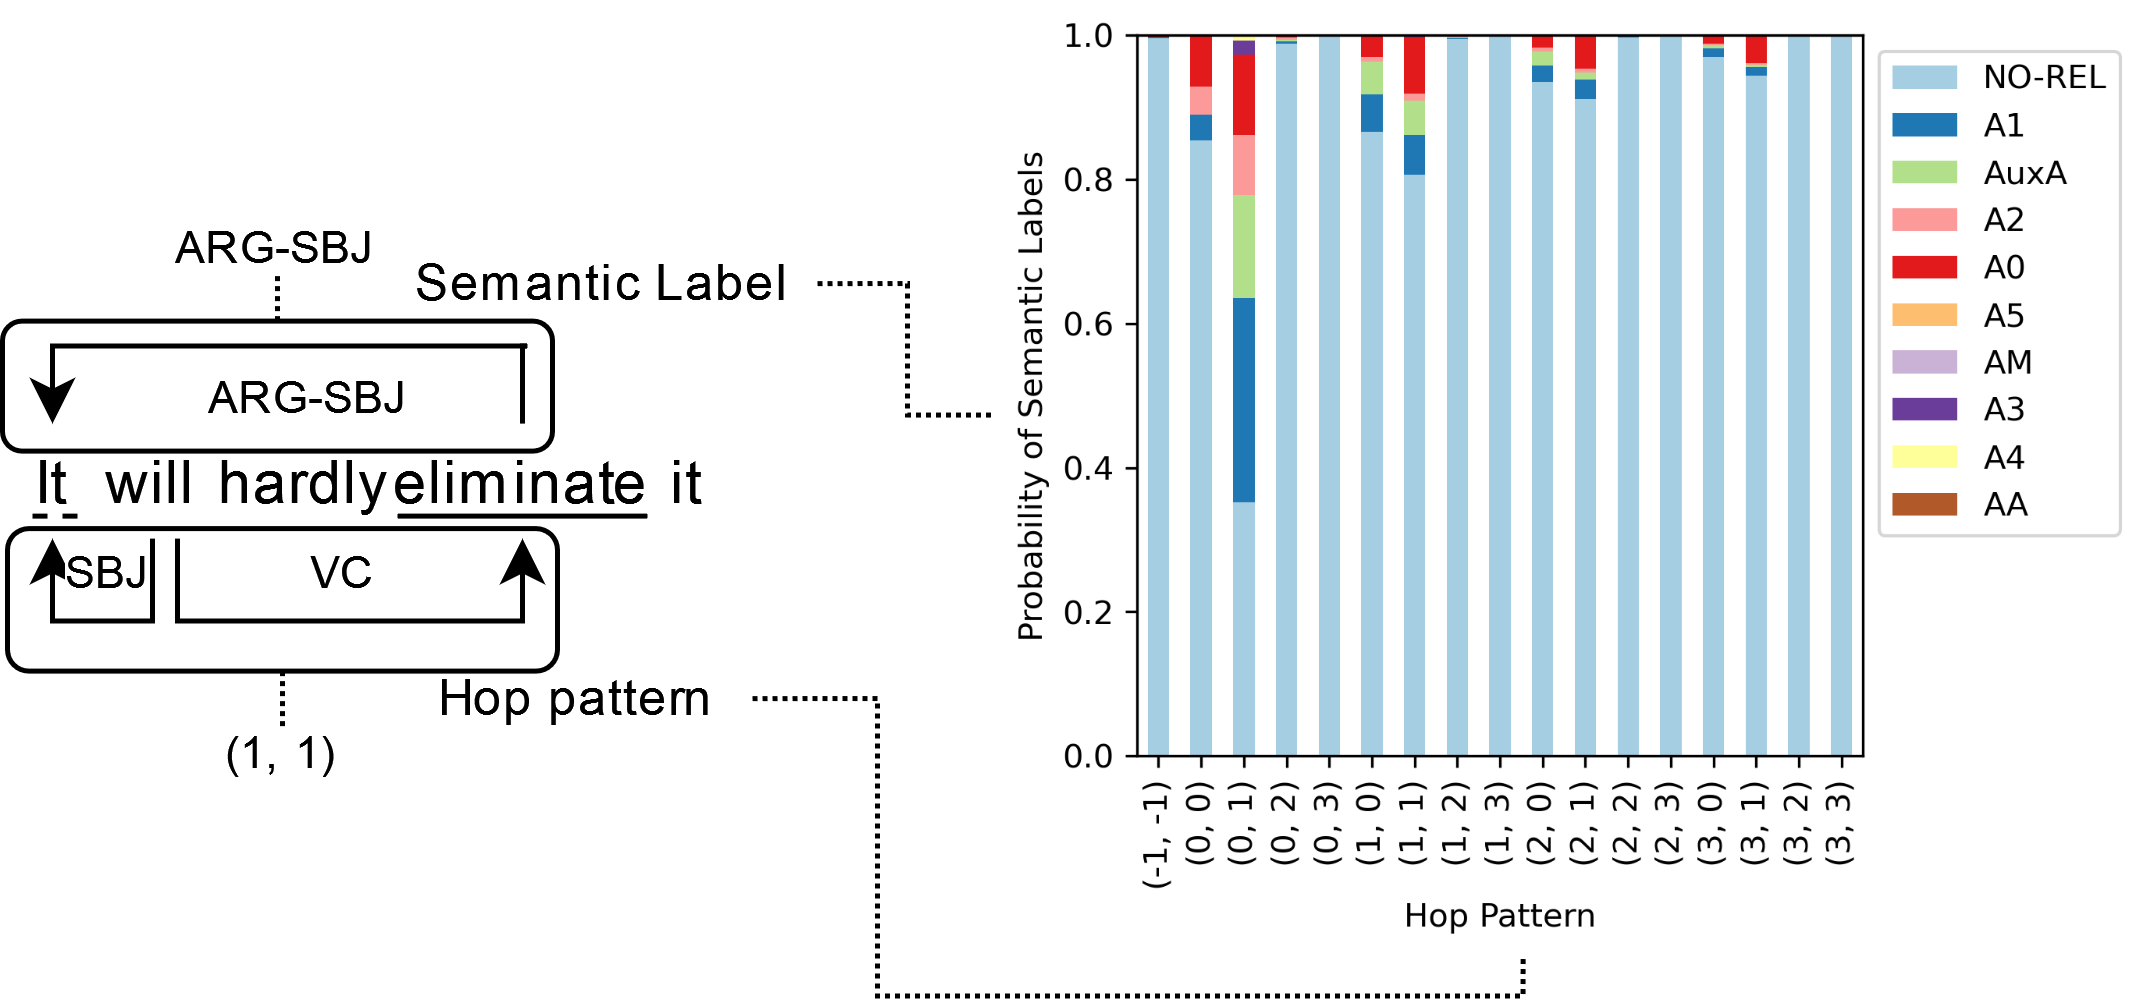
\includegraphics[width=\textwidth]{images/synsem-explanation-4.png}
    \vspace{-1.5\baselineskip}
    \caption{Semantic label distributions by hop patterns. (-1, -1) indicates hop patterns beyond (3, 3).}
    \label{fig:my_label}
\end{figure}
\end{columns}

\end{block}
    \vspace{-.2\baselineskip}
    \begin{alertblock}{Mutual Information Gain of Hop Patterns}
Mutual information gain measures the impact of hop patterns on semantic label distributions\\
\vspace{0.5cm}
{
\begin{column}{0.8\colwidth}
Analysis:
\begin{itemize}
    \item Hop pattern (0,1) has the highest information gain of 0.149bits
    \item Long hop patterns have near-zero information gains
    \item Short hop patterns have diverse non-zero information gains, ranging from 0.011 bits to 0.149bits
\end{itemize}
% \begin{itemize}
% % \vspace{0.8cm}
%     \item $X$: syntactic variable mapping predicate-argument pairs to their hop patterns
%     \begin{itemize}
%         \item $X_{(\alpha, \beta)}$: syntax-aware model sensitive to the hop pattern $X_{(\alpha, \beta)}$
%         \item $X_0$: syntax-agnostic model
%     \end{itemize}
%     \item $Y$: semantic variable mapping predicate-argument pairs to their semantic labels
        
%     \item $\Delta \mathrm{MI}(X_{(\alpha, \beta)}, X_0):=\mathrm{MI}(X_{(\alpha, \beta)}, Y) - \mathrm{MI}(X_0, Y)$
% \end{itemize}
\end{column}
\begin{column}{1.1\colwidth}
\begin{figure}
    \centering
    \captionsetup{justification=centering}
    \vspace{-1cm}
    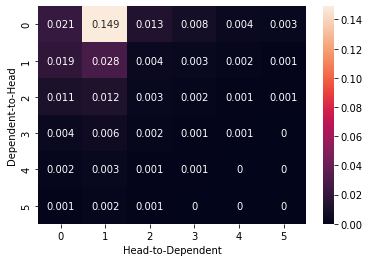
\includegraphics[width=0.75\textwidth]{images/ssdp-mi.png}
    \vspace{-0.5cm}
\caption{Mutual information gain of hop patterns up to (5, 5)}
    \label{fig:my_label}
\end{figure}
% \vspace{3cm}

\end{column}
}
\\
% {
%     \begin{align}
%     X_{(\alpha, \beta)}(p^s, a^s)&=\begin{cases}
%     1, (p^s, a^s)\text{ is of }(\alpha, \beta)\\
%     0, \text{otherwise}
%     \end{cases}\label{eq-rvsyn-aware}\\
%     X_0(p^s, a^s) &= 0\label{eq-rvsyn-agnostic}\\
%     \Delta \mathrm{MI}(X_{(\alpha, \beta)}, X_0) &= \mathrm{MI}(X_{(\alpha, \beta)}, Y) - \mathrm{MI}(X_0, Y) 
%     \label{eq-deltami}
%     \end{align}
% }
\vspace{-1.5cm}
{
\begin{column}{0.8\colwidth}
\begin{figure}
    \vspace{-3.2cm}
    % \RaggedLeft 
    
\includegraphics[width=0.3\textwidth]{images/agreement arrow.drawio.png}
    % \caption{Caption}
    % \label{fig:my_label}
\end{figure}
% \vspace{1cm}
Results:
\begin{itemize}
    \item Models assign a unique component to the hop pattern (0, 1), the hop pattern with the highest information gain
    \item Models assign long SSDPs with near-zero information gains to a single component
    \item Models assign SSDPs with diverse information gains to different components
\end{itemize}
\end{column}
% \separatorcolmun
\begin{column}{1.1\colwidth}
\begin{table}[]
\vspace{1cm}
\captionsetup{justification=centering}
\small
\centering
\begin{subtable}{0.3\textwidth}
\centering
\begin{tabular}{|l|r|r|r|r|} 
\hline
\backslashbox{$\alpha$}{$\beta$} & 0 & 1 & 2 & 3  \\ 
\hline
0 & \cellcolor{purple}3 & \cellcolor{white}1 & \cellcolor{gray}0 & \cellcolor{gray}0 \\ \hline
1 & \cellcolor{violet}2 & \cellcolor{violet}2 & \cellcolor{gray}0 & \cellcolor{gray}0 \\ \hline
2 & \cellcolor{violet}2 & \cellcolor{violet}2 & \cellcolor{gray}0 & \cellcolor{gray}0 \\ \hline
3 & \cellcolor{violet}2 & \cellcolor{gray}0 & \cellcolor{gray}0 & \cellcolor{gray}0 \\ \hline
4 & \cellcolor{gray}0 & \cellcolor{gray}0 & \cellcolor{gray}0 & \cellcolor{gray}0 \\ \hline
5 & \cellcolor{gray}0 & \cellcolor{gray}0 & \cellcolor{gray}0 & \cellcolor{gray}0 \\ \hline
\end{tabular}
% \vspace{0.5cm}
\subcaption{FastText}
% \label{tbl-cluster_assignment-glove}
\end{subtable}
\quad
\begin{subtable}{0.3\textwidth}
\centering
\begin{tabular}{|l|r|r|r|r|} 
\hline
\backslashbox{$\alpha$}{$\beta$} & 0 & 1 & 2 & 3  \\ 
\hline
0 & \cellcolor{purple}2 & \cellcolor{white}0 & \cellcolor{gray}4 & \cellcolor{gray}4 \\ \hline
1 & \cellcolor{purple}2 & \cellcolor{violet}1 & \cellcolor{gray}4 & \cellcolor{gray}4 \\ \hline
2 & \cellcolor{cyan}\cellcolor{cyan}3 & \cellcolor{cyan}3 & \cellcolor{gray}4 & \cellcolor{gray}4 \\ \hline
3 & \cellcolor{gray}4 & \cellcolor{gray}4 & \cellcolor{gray}4 & \cellcolor{gray}4 \\ \hline
4 & \cellcolor{gray}4 & \cellcolor{gray}4 & \cellcolor{gray}4 & \cellcolor{gray}4 \\ \hline
5 & \cellcolor{gray}4 & \cellcolor{gray}4 & \cellcolor{gray}4 & \cellcolor{gray}4 \\ \hline
\end{tabular}
% \vspace{0.5cm}
\subcaption{ELMo}
% \label{tbl-cluster_assignment-glove}
\end{subtable}
\quad
\begin{subtable}{0.3\textwidth}
\centering
\begin{tabular}{|l|r|r|r|r|}
\hline
\backslashbox{$\alpha$}{$\beta$} & 0 & 1 & 2 & 3 \\ \hline
0 & \cellcolor{purple}4 & \cellcolor{white}0 & \cellcolor{gray}2 & \cellcolor{gray}2 \\ \hline
1 & \cellcolor{purple}4 & \cellcolor{violet}3 & \cellcolor{gray}2 & \cellcolor{gray}2 \\ \hline
2 & \cellcolor{purple}4 & \cellcolor{violet}3 & \cellcolor{gray}2 & \cellcolor{gray}2 \\ \hline
3 & \cellcolor{purple}4 & \cellcolor{purple}4 & \cellcolor{gray}2 & \cellcolor{gray}2 \\ \hline
4 & \cellcolor{gray}2 & \cellcolor{gray}2 & \cellcolor{gray}2 & \cellcolor{gray}2 \\ \hline
5 & \cellcolor{gray}2 & \cellcolor{gray}2 & \cellcolor{gray}2 & \cellcolor{gray}2 \\ \hline
\end{tabular}
% \vspace{0.5cm}
\caption{BERT}
% \label{tbl-cluster_assignment-elmo}
\end{subtable}
\vspace{-0.5cm}
\caption{Component assignments extracted from models}
\label{tbl:cluster-assignment}
\end{table}
\end{column}
}

\textbf{Conclusion: \colorbox{yellow}{Semantic label distributions of different hop patterns have unique properties}}

\end{alertblock}
    % % \vspace{}
\begin{block}{Proposal Derivation}
\begin{column}{1.99\colwidth}
% We optimize the mixture model through the Evidence Lowerbound objective (ELBo) $\mathcal{L}_{sem}(\theta)$\\
    % \vspace{0.8cm}
Assumptions to derive the Evidence Lowerbound objective $\mathcal{L}_{sem}(\theta)$ from the log-likelihood of semantic labels:
\begin{enumerate}
\vspace{-0.3cm}
    \item Predicate-argument pairs and hop patterns determine semantic labels
    \item Cluster assignments are determined only by hop patterns
\end{enumerate}
    \end{column}
    % \small
    % \vspace{-1cm}
    \begin{flalign}
       && \log P_\theta(r|p, a)&= \log\sum_c P_\theta(r|c, p, a)P_\theta(c|p, a) &&\nonumber \\
       &&                     &\geq \sum_c q_\phi(c|r, p, a)\log\frac{P_\theta(r|c, p, a)P_\theta(c|p, a)}{q_\phi(c|r, p, a)} && \text{ELBo inequality}\nonumber\\
       &&                    &=\sum_c q_\phi(c|p, a)\log\frac{P_\theta(r|c, p, a)P_\theta(c|p, a)}{q_\phi(c|p, a)} && \text{Using assumption 1}\nonumber\\
       &&                     &=\sum_c P_\theta(c|\mathrm{ssdp}(p, a))\log\frac{P_\theta(r|c, p, a)P_\theta(c|\mathrm{ssdp}(p, a))}{P_\theta(c|\mathrm{ssdp}(p, a))} && \text{Using assumption 2}\nonumber\\
        &&                    &= \sum_c P_\theta(c|\mathrm{ssdp}(p, a)) \log P_\theta(r|c, p, a)= \mathcal{L}_{sem}(\theta|\mathcal{X}=(r, p, a)) &&\nonumber 
    \end{flalign}
\end{block}
    \vspace{-.2\baselineskip}
    \begin{exampleblock}{CoNLL-2009 Experiments}

\begin{column}{0.85\colwidth}
% \vspace{1cm}
% Experiments on CoNLL-2009
% \vspace{0.2cm}
MM outperforms baseline methods in most cases
% \vspace{1cm}
\begin{itemize}
    \item MM outperforms baselines over FastText, ELMo, and Bert embeddings (Figure. \ref{fig:perf-emb})
    \item MM outperforms baselines over many languages (Figure. \ref{fig:perf-multilingual})
    \begin{itemize}
        \item MM outperforms Multitask and Transformer in German, Spanish, and Catalan
        \item MM outperforms Transformer in Chinese
        \item MM fails to learn in Czech
    \end{itemize}
\item MM improves in predicting short-distance semantic dependencies (Figure. \ref{fig:perf-by-ll})
    \begin{itemize}
        \item MM is the only syntax-aware method improving over Transformer on FastText and ELMo embeddings
        \item MM retains the advantage in long-distance semantic dependencies of syntax-aware methods
    \end{itemize}
\end{itemize}

\begin{table}[]
\centering
\small
\begin{tabular}{l|c||l|c}
\toprule
Method & Syntax-aware & Method & Syntax-aware  \\
\midrule
Transformer   & No  &  Multitask       & Yes   \\
LISA\cite{strubell-etal-2018-linguistically}     & Yes & PathLSTM\cite{roth-lapata-2016-neural}   & Yes  \\
Pruning\cite{he-etal-2018-syntax} & Yes & MM & Yes \\
\bottomrule
\end{tabular}
\caption{List of methods}
\end{table}

\end{column}
\begin{column}{1.1\colwidth}
\begin{figure}
\vspace{-1cm}
\captionsetup{justification=centering}
    \centering
    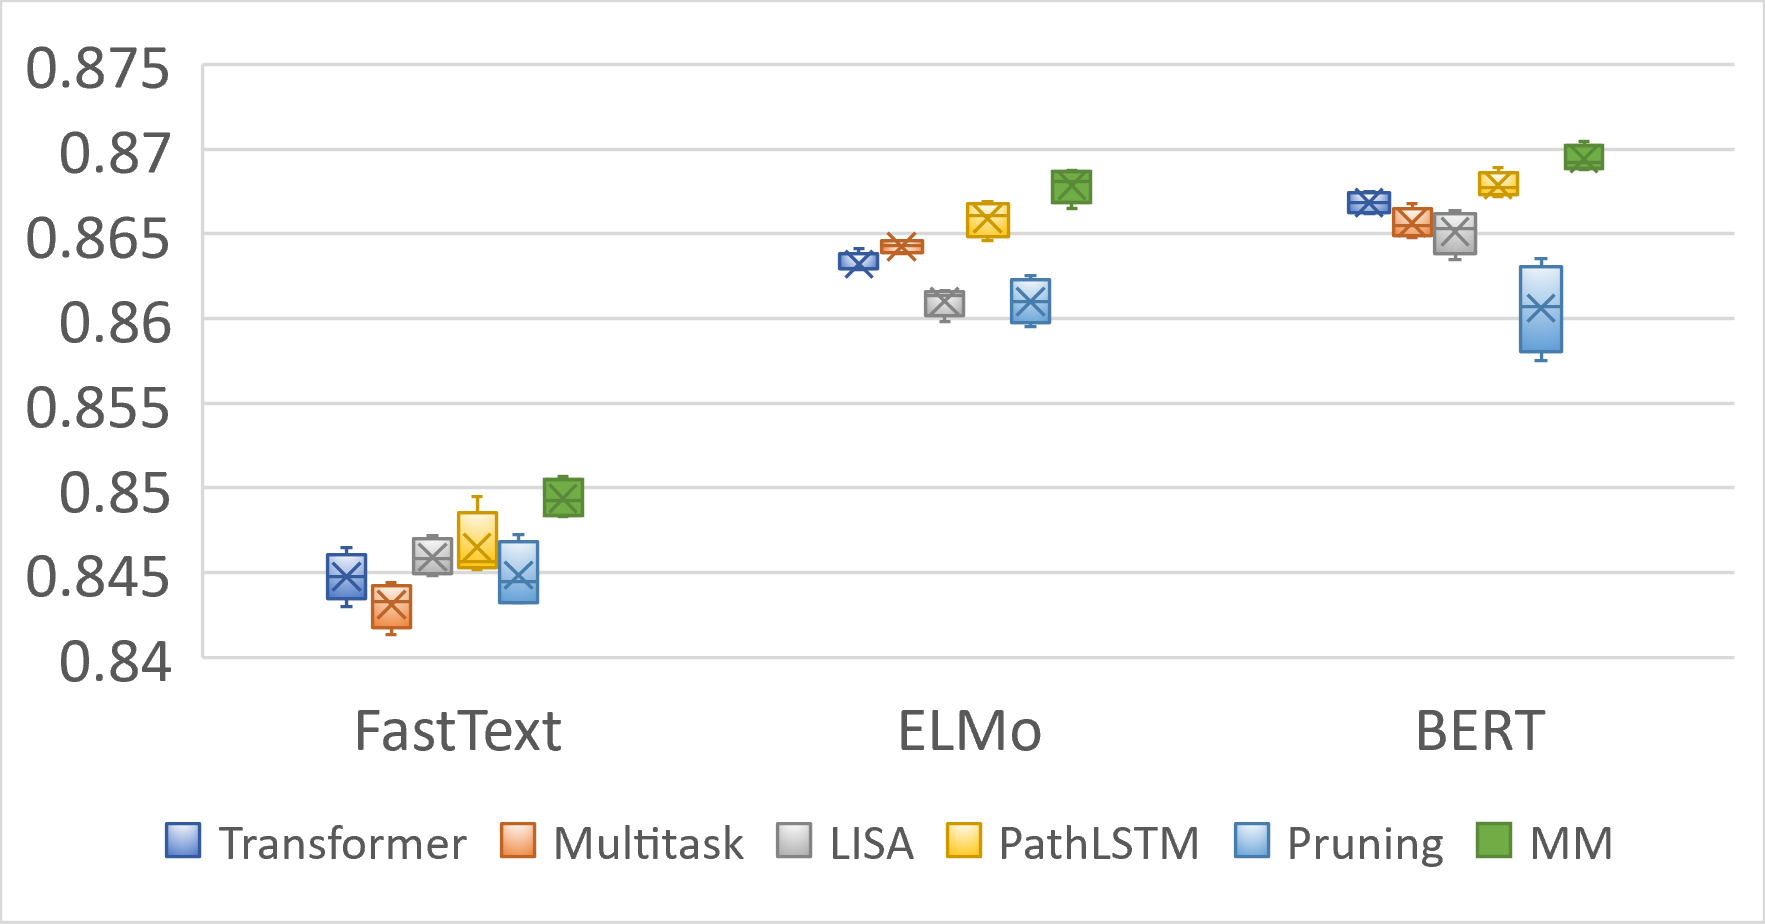
\includegraphics[width=0.85\textwidth]{images/poster-perf-english-by-embeddings.png}
    \caption{English LAS comparison on input embeddings.}
    \label{fig:perf-emb}
\end{figure}
\begin{figure}
\captionsetup{justification=centering}
    \centering
    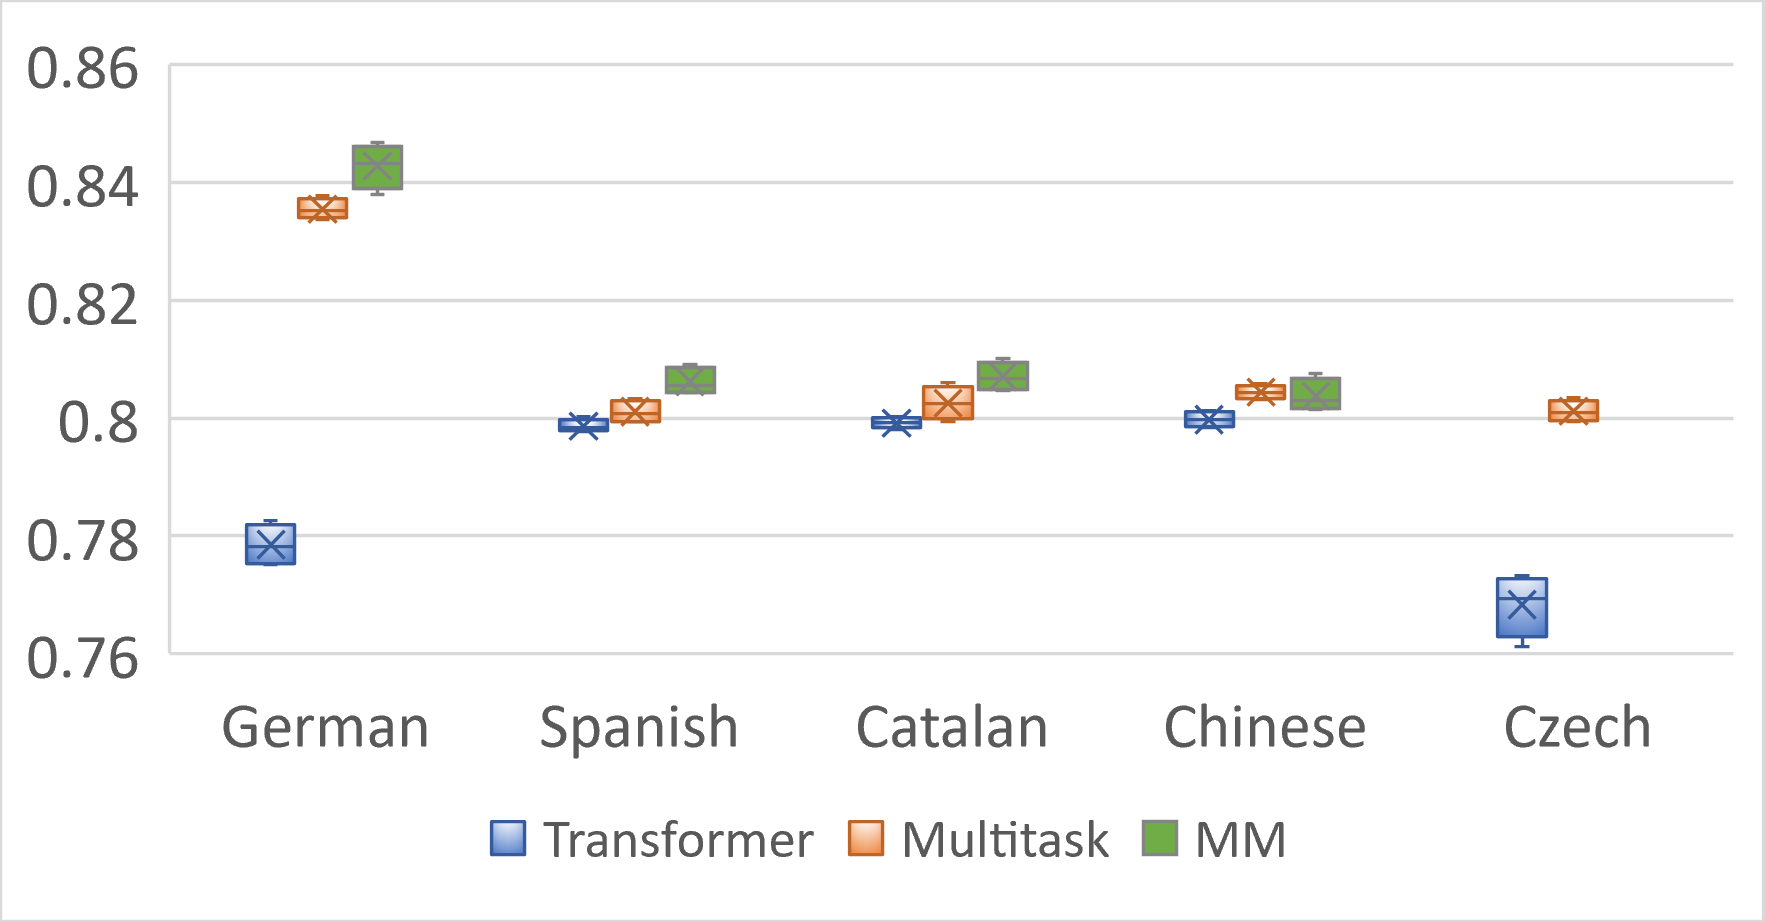
\includegraphics[width=0.85\textwidth]{images/poster-perf-multilingual.png}
    \caption{LAS comparison on five languages using FastText.}
    \label{fig:perf-multilingual}
\end{figure}

\end{column}

\begin{figure}
    \centering
    \captionsetup{justification=centering}
    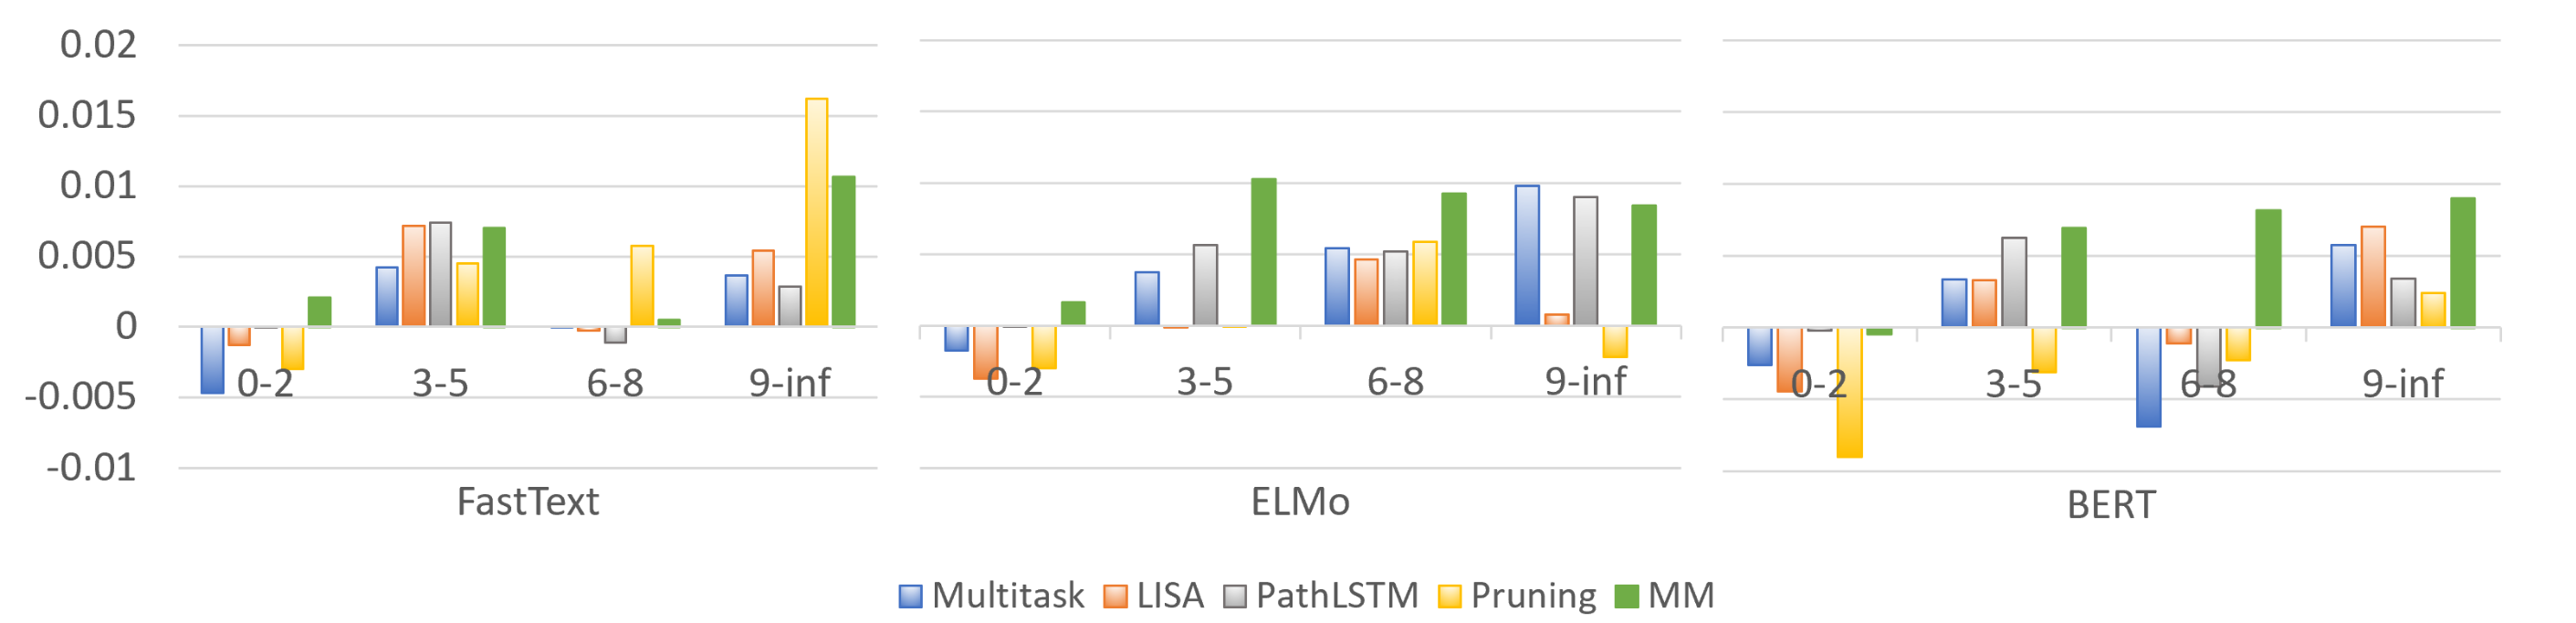
\includegraphics[width=0.9\textwidth]{images/perf-by-ll.drawio.png}
    \caption{Relative LAS comparison by the linear distance of semantic dependencies (English, FastText). }
    \label{fig:perf-by-ll}
\end{figure}


\end{exampleblock}
    % % \vspace{}
\begin{block}{Proposal Derivation}
\begin{column}{1.99\colwidth}
% We optimize the mixture model through the Evidence Lowerbound objective (ELBo) $\mathcal{L}_{sem}(\theta)$\\
    % \vspace{0.8cm}
Assumptions to derive the Evidence Lowerbound objective $\mathcal{L}_{sem}(\theta)$ from the log-likelihood of semantic labels:
\begin{enumerate}
\vspace{-0.3cm}
    \item Predicate-argument pairs and hop patterns determine semantic labels
    \item Cluster assignments are determined only by hop patterns
\end{enumerate}
    \end{column}
    % \small
    % \vspace{-1cm}
    \begin{flalign}
       && \log P_\theta(r|p, a)&= \log\sum_c P_\theta(r|c, p, a)P_\theta(c|p, a) &&\nonumber \\
       &&                     &\geq \sum_c q_\phi(c|r, p, a)\log\frac{P_\theta(r|c, p, a)P_\theta(c|p, a)}{q_\phi(c|r, p, a)} && \text{ELBo inequality}\nonumber\\
       &&                    &=\sum_c q_\phi(c|p, a)\log\frac{P_\theta(r|c, p, a)P_\theta(c|p, a)}{q_\phi(c|p, a)} && \text{Using assumption 1}\nonumber\\
       &&                     &=\sum_c P_\theta(c|\mathrm{ssdp}(p, a))\log\frac{P_\theta(r|c, p, a)P_\theta(c|\mathrm{ssdp}(p, a))}{P_\theta(c|\mathrm{ssdp}(p, a))} && \text{Using assumption 2}\nonumber\\
        &&                    &= \sum_c P_\theta(c|\mathrm{ssdp}(p, a)) \log P_\theta(r|c, p, a)= \mathcal{L}_{sem}(\theta|\mathcal{X}=(r, p, a)) &&\nonumber 
    \end{flalign}
\end{block}
    %   \begin{block}{References}

    % \nocite{*}
    \footnotesize{\bibliographystyle{plain}\bibliography{anthology}}

  \end{block}
% % \vspace{}
\begin{block}{Proposal Derivation}
\begin{column}{1.99\colwidth}
% We optimize the mixture model through the Evidence Lowerbound objective (ELBo) $\mathcal{L}_{sem}(\theta)$\\
    % \vspace{0.8cm}
Assumptions to derive the Evidence Lowerbound objective $\mathcal{L}_{sem}(\theta)$ from the log-likelihood of semantic labels:
\begin{enumerate}
\vspace{-0.3cm}
    \item Predicate-argument pairs and hop patterns determine semantic labels
    \item Cluster assignments are determined only by hop patterns
\end{enumerate}
    \end{column}
    % \small
    % \vspace{-1cm}
    \begin{flalign}
       && \log P_\theta(r|p, a)&= \log\sum_c P_\theta(r|c, p, a)P_\theta(c|p, a) &&\nonumber \\
       &&                     &\geq \sum_c q_\phi(c|r, p, a)\log\frac{P_\theta(r|c, p, a)P_\theta(c|p, a)}{q_\phi(c|r, p, a)} && \text{ELBo inequality}\nonumber\\
       &&                    &=\sum_c q_\phi(c|p, a)\log\frac{P_\theta(r|c, p, a)P_\theta(c|p, a)}{q_\phi(c|p, a)} && \text{Using assumption 1}\nonumber\\
       &&                     &=\sum_c P_\theta(c|\mathrm{ssdp}(p, a))\log\frac{P_\theta(r|c, p, a)P_\theta(c|\mathrm{ssdp}(p, a))}{P_\theta(c|\mathrm{ssdp}(p, a))} && \text{Using assumption 2}\nonumber\\
        &&                    &= \sum_c P_\theta(c|\mathrm{ssdp}(p, a)) \log P_\theta(r|c, p, a)= \mathcal{L}_{sem}(\theta|\mathcal{X}=(r, p, a)) &&\nonumber 
    \end{flalign}
\end{block}
\end{column}
\separatorcolumn

% \begin{column}{\colwidth}

%   \begin{exampleblock}{CoNLL-2009 Experiments}

\begin{column}{0.85\colwidth}
% \vspace{1cm}
% Experiments on CoNLL-2009
% \vspace{0.2cm}
MM outperforms baseline methods in most cases
% \vspace{1cm}
\begin{itemize}
    \item MM outperforms baselines over FastText, ELMo, and Bert embeddings (Figure. \ref{fig:perf-emb})
    \item MM outperforms baselines over many languages (Figure. \ref{fig:perf-multilingual})
    \begin{itemize}
        \item MM outperforms Multitask and Transformer in German, Spanish, and Catalan
        \item MM outperforms Transformer in Chinese
        \item MM fails to learn in Czech
    \end{itemize}
\item MM improves in predicting short-distance semantic dependencies (Figure. \ref{fig:perf-by-ll})
    \begin{itemize}
        \item MM is the only syntax-aware method improving over Transformer on FastText and ELMo embeddings
        \item MM retains the advantage in long-distance semantic dependencies of syntax-aware methods
    \end{itemize}
\end{itemize}

\begin{table}[]
\centering
\small
\begin{tabular}{l|c||l|c}
\toprule
Method & Syntax-aware & Method & Syntax-aware  \\
\midrule
Transformer   & No  &  Multitask       & Yes   \\
LISA\cite{strubell-etal-2018-linguistically}     & Yes & PathLSTM\cite{roth-lapata-2016-neural}   & Yes  \\
Pruning\cite{he-etal-2018-syntax} & Yes & MM & Yes \\
\bottomrule
\end{tabular}
\caption{List of methods}
\end{table}

\end{column}
\begin{column}{1.1\colwidth}
\begin{figure}
\vspace{-1cm}
\captionsetup{justification=centering}
    \centering
    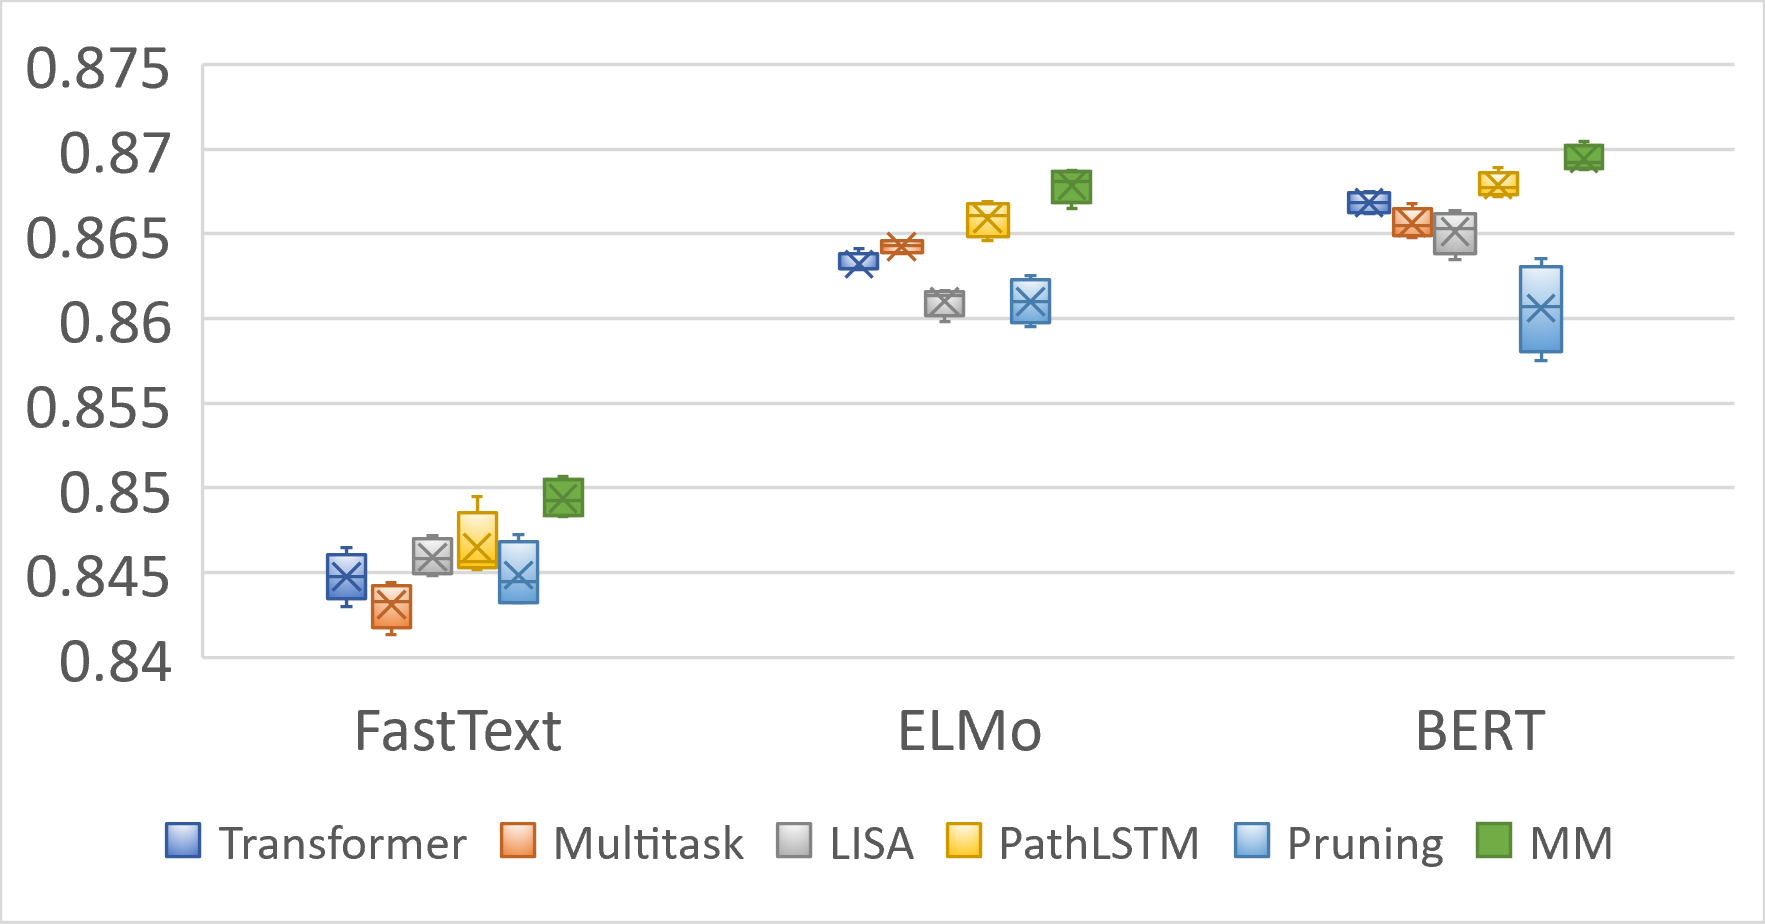
\includegraphics[width=0.85\textwidth]{images/poster-perf-english-by-embeddings.png}
    \caption{English LAS comparison on input embeddings.}
    \label{fig:perf-emb}
\end{figure}
\begin{figure}
\captionsetup{justification=centering}
    \centering
    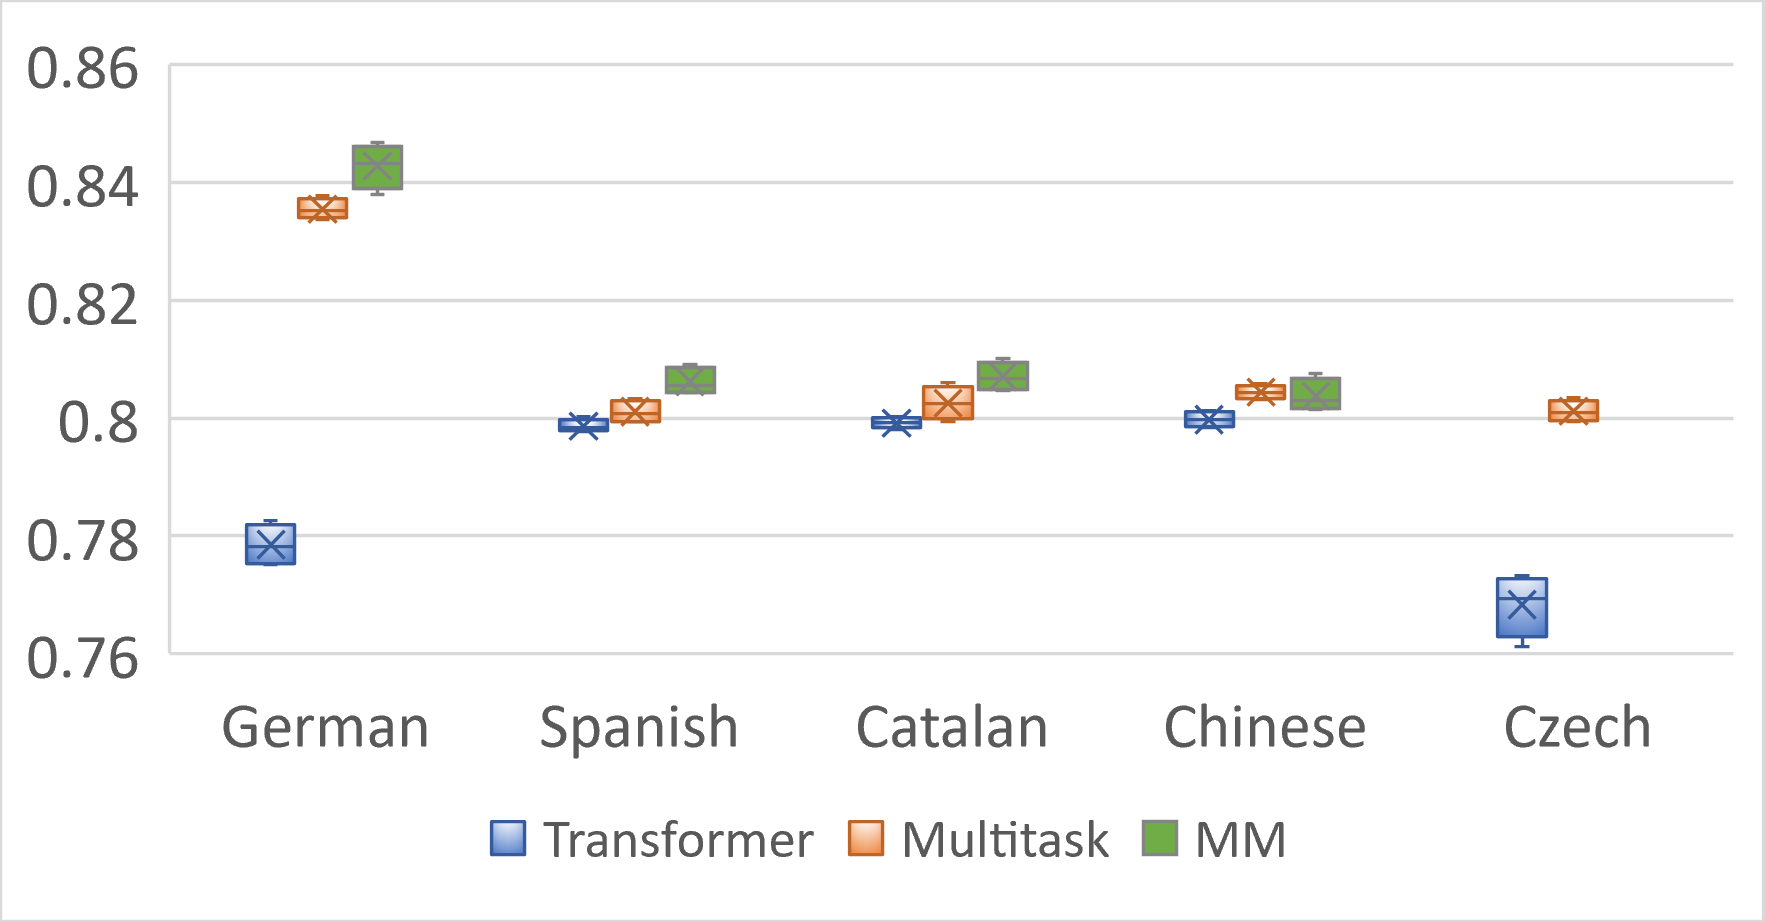
\includegraphics[width=0.85\textwidth]{images/poster-perf-multilingual.png}
    \caption{LAS comparison on five languages using FastText.}
    \label{fig:perf-multilingual}
\end{figure}

\end{column}

\begin{figure}
    \centering
    \captionsetup{justification=centering}
    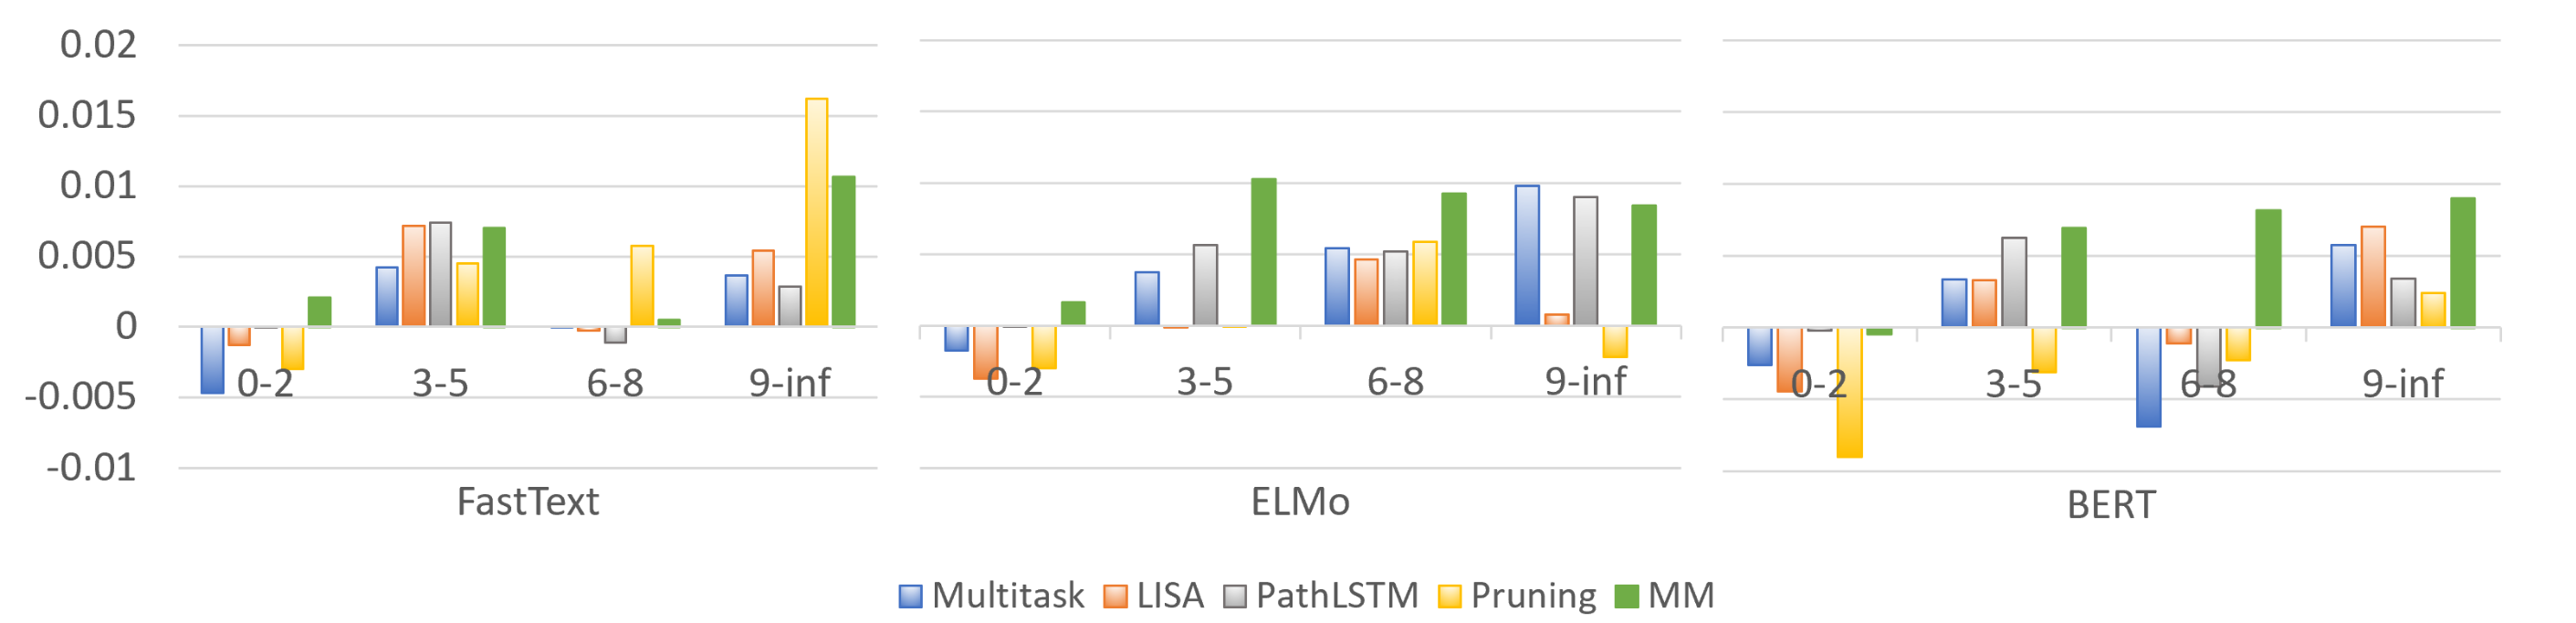
\includegraphics[width=0.9\textwidth]{images/perf-by-ll.drawio.png}
    \caption{Relative LAS comparison by the linear distance of semantic dependencies (English, FastText). }
    \label{fig:perf-by-ll}
\end{figure}


\end{exampleblock}

%   \begin{block}{References}

%     \nocite{*}
%     \footnotesize{\bibliographystyle{plain}\bibliography{poster}}

%   \end{block}

% \end{column}

\separatorcolumn
\end{columns}
\end{frame}

\end{document}
